% ======================================================================
%  A Two-Channel Accretion Mechanism for Evolving Dark Energy
%  Christopher P. Green  —  Independent Researcher
%  Compile: pdflatex -> bibtex -> pdflatex -> pdflatex  (or latexmk -pdf)
% ======================================================================
\documentclass[11pt,a4paper]{article}

\usepackage[margin=2.6cm]{geometry}
\usepackage{amsmath,amssymb}
\usepackage{graphicx}
\usepackage{booktabs}
\usepackage{makecell}
\usepackage[expansion=false]{microtype}
\usepackage[numbers,sort&compress]{natbib}
\usepackage{url}
\usepackage{xcolor}
\definecolor{linkblue}{RGB}{25,50,120}
\usepackage[colorlinks=true,linkcolor=linkblue,citecolor=linkblue,urlcolor=linkblue]{hyperref}

\setlength{\emergencystretch}{2.2em}

\newcommand{\lcdm}{\ensuremath{\Lambda}CDM}
\newcommand{\weff}{w_{\rm eff}}

\title{\bfseries A Two-Channel Accretion Mechanism for\\ Evolving Dark Energy}
\author{Christopher P. Green\\[2pt]
\normalsize\itshape Independent Researcher\\[2pt]
\normalsize\upshape\texttt{research@wilson-green.com}}
\date{July 2026}

\begin{document}

\maketitle

\begin{abstract}
\noindent
We present a physical mechanism for the evolving dark-energy signal reported in recent combined DESI analyses. The mechanism consists of two competing contributions driven by a single accretion flux onto a parent black hole whose interior is the observable universe: energy delivered inward across the one-way horizon, a fraction $\kappa$ of which converts to interior vacuum energy (raising $\rho_{\rm de}$), and growth of the horizon itself, which enlarges the interior and dilutes that vacuum. Because the injection spreads over the interior's physical volume ($\propto a^3$) while the dilution tracks the boundary, the injection dominates early and the dilution late: the dark-energy density rises, peaks, and declines, and the effective equation of state crosses $w=-1$ from below --- phantom-like in the past, quintessence-like today --- with no phantom fields, through the standard signature of energy injection into the dark sector. Fit against Planck CMB distance priors, DESI BAO, and the full Pantheon+ supernova sample (1580 SNe, complete systematic covariance), the model attains $\chi^2=1403.3$: statistically identical to the empirical $w_0$--$w_a$ parameterisation (1403.4) and $\Delta\chi^2\simeq6$ below \lcdm{} (1409.4), with the crossing at $z\simeq0.40$, the density peak at $z\simeq0.40$, $w\simeq-0.86$ today, and a fitted conversion efficiency $\kappa\simeq0.85$ --- inside the physical energy budget. The rise--peak--decline ordering is not fitted: for $\kappa\le1$ the model provably cannot place the phantom phase in the present, and no parameter choice yields the reverse history. The dilution channel coincides exactly with the Misner--Sharp horizon relation and the injection accounting follows the Oppenheimer--Snyder matching; the junction analysis for an actively fed (Vaidya-type) boundary and the perturbation-level treatment remain open. A further feature distinguishes the mechanism from a pure equation-of-state fit: because the boundary is a temporal surface, uneven or rotating accretion breaks global isotropy in the interior, offering a natural route to the large-scale directional anomalies seen in the CMB --- a connection developed in \S\ref{sec:speculative} rather than fitted here. The model makes one central bet --- that the evolving-dark-energy preference --- $\sim2\sigma$ on the data vector fitted here, since strengthened to $2.8$--$4.2\sigma$ by DESI's second data release, depending on the supernova sample --- is real and has this shape --- and fails with it if future surveys converge on \lcdm{}.
\end{abstract}

% ----------------------------------------------------------------------
\section{Introduction}\label{sec:intro}

Combined analyses of DESI baryon-acoustic-oscillation data with the cosmic microwave background and Type Ia supernovae currently prefer an evolving dark energy over a cosmological constant: at the $3.1\sigma$ level for DESI DR2 BAO combined with the CMB, rising to $2.8$--$4.2\sigma$ when supernovae are added, depending on the sample used \citep{DESI_DR1,DESI_DR2}. The completed five-year survey (more than 47 million galaxies and quasars, with observations extended to 2028) is under analysis, with first full-survey dark-energy results expected in 2027 \citep{DESI_completion}. The preferred $w_0$--$w_a$ fits \citep{ChevallierPolarski2001,Linder2003} describe a dark energy that was phantom-like in the past ($w<-1$), crossed $w=-1$ near $z\sim0.4$, and is quintessence-like today \citep{DESI_DR2} --- a history that is awkward to realise: fundamental phantom fields are widely regarded as pathological \citep{Caldwell2002,CarrollHoffmanTrodden2003}, and models that cross $w=-1$ typically do so by construction rather than for a physical reason. The signal therefore sits between two readings: an artifact of the two-parameter form, or new physics with no accepted mechanism.

This paper supplies a candidate mechanism in which that specific history is forced rather than fitted, and reports its confrontation with data. Against Planck distance priors, DESI BAO, and the full Pantheon+ sample, the mechanism matches the empirical $w_0$--$w_a$ description to within rounding ($\chi^2$ of 1403.3 versus 1403.4, against 1409.4 for \lcdm{}) --- it captures the entire measured preference for evolving dark energy --- while its crossing redshift, density peak, and present-day $w$ emerge as outputs, not inputs, and its single bounded parameter, an energy-conversion efficiency, is selected by the data at $\kappa\simeq0.85$, within the physical budget of $\kappa\le1$.

The mechanism arises within a black-hole-interior cosmology: the observable universe is modelled as the interior of a black hole embedded in a parent spacetime and fed by ongoing accretion. Section~\ref{sec:setting} states the geometric premises. The mechanism's two channels are individually established physics --- one is a geometric identity, the other a published conversion process --- and the data confrontation of Sections~\ref{sec:data}--\ref{sec:artifacts} is independent of the geometric interpretation. Section~\ref{sec:matching} presents the supporting matching arguments, Section~\ref{sec:prior} the relation to prior work, Section~\ref{sec:speculative} the consequences that follow from the geometric setting rather than from the fitted mechanism, and Section~\ref{sec:conclusion} the decisive tests.

The proposal is falsifiable at both ends. If the strict junction analysis for a fed boundary overturns the volume accounting of Section~\ref{sec:matching}, the mechanism fails theoretically. If the evolving-dark-energy signal dissolves as surveys mature, it fails empirically. It is stated precisely enough to lose.

% ----------------------------------------------------------------------
\section{Geometric setting}\label{sec:setting}

Four premises define the setting. The first two are familiar from the black-hole-cosmology literature; the third and fourth generate the mechanism.

\textbf{(i) The universe as a black-hole interior.} That the observable universe's mass and size satisfy a relation close to the Schwarzschild condition has been noted for decades \citep{Pathria1972}, and interior cosmological solutions --- collapse halting at extreme density and rebounding into an expanding interior --- are an established line of work in general relativity and its torsion-extended variants \citep{NovelloBergliaffa2008,Poplawski2010}. The ``Big Bang'' is a bounce inside a horizon, not a beginning from nothing.

\textbf{(ii) Ordinary matter fixed early.} Big-bang nucleosynthesis and the CMB tightly fix the early matter content \citep{Fields2020,Planck2018}. The interior baryonic and dark matter are established early and subsequently only dilute; the late-time channel below feeds the dark-energy sector only.

\textbf{(iii) A one-way horizon delivering accretion inward.} The interior's boundary is the parent's event horizon: nothing exits, and matter the parent accretes crosses inward. Inside a horizon the causal roles of the radial and time coordinates exchange, so infall is directed toward the interior's future. A fraction $\kappa$ of the infalling rest energy converts, on arrival, into interior vacuum energy: the \textbf{injection} channel.

\textbf{(iv) The same feeding grows the container.} Accretion grows the parent's mass and horizon, enlarging the interior and diluting its vacuum: the \textbf{dilution} channel. With injection switched off ($\kappa=0$) this limit can only weaken the dark energy, forcing $w\ge-1$ at all times; it serves below as the reduced model.

The essential content is that (iii) and (iv) are two channels driven by the same flux, with opposite signs and different volume dependence --- injection into the interior's expanding volume ($\propto a^3$), dilution tied to the boundary. Their competition evolves: injection dominates while the universe is small, dilution as it grows. Dark energy strengthens, peaks, and weakens, in that order only.

% ----------------------------------------------------------------------
\section{The model}\label{sec:model}

\subsection{Background equations}\label{sec:background}

For a spatially flat FRW interior with $a_0=1$ today:
\begin{equation}
H^2(a)=\frac{8\pi G}{3}\big[\rho_{\rm m}(a)+\rho_{\rm r}(a)+\rho_{\rm de}(a)\big],
\label{eq:friedmann}
\end{equation}
with $\rho_{\rm m}\propto a^{-3}$, $\rho_{\rm r}\propto a^{-4}$. The new physics resides in $\rho_{\rm de}$.

\subsection{Feeding history}\label{sec:feeding}

With $M_p(a)$ the parent's mass, non-decreasing because feeding is one-way, the fractional feeding rate is parametrised as
\begin{equation}
\frac{d\ln M_p}{d\ln a}=\mu_0\,a^{\,n},\qquad \mu_0\ge 0,
\label{eq:feeding}
\end{equation}
giving $M_p(a)=M_p(1)\exp\!\big[-\mu_0(1-a^{n})/n\big]$. The pair $(\mu_0,n)$ encodes the accretion history as seen from inside; Section~\ref{sec:matching} shows the same pair absorbs the parent-to-interior clock mapping.

\subsection{The two channels}\label{sec:channels}

In units of today's dark-energy density, $\rho\equiv\rho_{\rm de}/\rho_{\rm de,0}$:
\begin{equation}
\boxed{\ \frac{d\rho}{d\ln a}=\mu_0\,a^{\,n}\Big[\underbrace{\kappa\,\frac{M_p(a)/M_p(1)}{a^{3}}}_{\text{injection }(+)}\;-\;\underbrace{2\,\rho}_{\text{dilution }(-)}\Big].\ }
\label{eq:master}
\end{equation}
The prefactor is the feeding rate: neither channel operates when the parent is not feeding. The injection term is the converted infall energy $\kappa\,\dot M_p c^2$ shared over the interior's physical volume, hence $a^{-3}$, with $\kappa\le1$ on energy grounds. The dilution coefficient is not adjustable: it follows from the horizon slaving $\rho\propto M^{-2}$ derived in Section~\ref{sec:matching}, which this term reproduces exactly when $\kappa=0$.

\subsection{The forced ordering}\label{sec:ordering}

The effective equation of state is $\weff=-1-\tfrac13\,d\ln\rho/d\ln a$: phantom-like while injection dominates (density rising), quintessence-like while dilution dominates (density falling), with a crossing of $w=-1$ from below at the handover.

The ordering of the phases is a theorem of the model, not a fit outcome. At the present epoch, with $\rho(1)=1$ and $M_p(a)/M_p(1)=1$, the bracket evaluates to $\kappa-2$: for any $\kappa<2$ --- and physically $\kappa\le1$ --- and any $\mu_0>0$, the density is declining \emph{today} and $\weff(0)>-1$ strictly. Any phantom phase is confined to the past, where the $a^{-3}$ factor can lift the injection above the dilution. No parameter choice with $\mu_0\ge0$, $\kappa\le1$ produces the reverse history (quintessence past, phantom present). The model can therefore fail against data that prefer the reverse ordering, and could never have been tuned to accommodate it.

The phantom phase involves no phantom matter. No component has superluminal or negative-kinetic-energy character; the apparent $w<-1$ is the standard signature of energy injection into the dark sector, familiar from interacting-dark-energy models \citep{DasCorasanitiKhoury2006,Wang2016}. The one-way horizon --- which for $\kappa=0$ forbids $w<-1$, the wall only moving outward --- is precisely what permits the phantom appearance: the flux is inward, an injection, and injection mimics phantom.

\subsection{Energy conditions and the covariant completion}\label{sec:energyconditions}

The model is phenomenological: it is defined by the sourced continuity equation of \S\ref{sec:channels}, not derived from an action, and no explicit Lagrangian for the conversion vertex is claimed --- a status shared with the published cosmologically-coupled-black-hole programme, whose microphysical realisation is likewise contested \citep{CrokerWeiner2019,Croker2024,GaurVisser2024}. What can be established is the energy-condition budget of the minimal covariant completion, and that budget is clean.

Local conservation, enforced by the Einstein equations, forbids energy appearing in the dark sector ex nihilo: injected energy requires a physical carrier. The natural carrier is the infall itself --- an ingoing null flux of Vaidya type \citep{Vaidya1951}, $T_{\mu\nu}=\varepsilon\,k_\mu k_\nu$ with $k_\mu$ null and $\varepsilon\ge0$, crossing the horizon and converting to vacuum energy in the interior. Every component then satisfies the weak energy condition pointwise: the null dust by construction, the vacuum term $T_{\mu\nu}=-\rho_{\rm de}\,g_{\mu\nu}$ because $\rho_{\rm de}\ge0$ (a positive density that the injection \emph{raises}), matter and radiation trivially. The null energy condition is nowhere violated --- the vacuum saturates it and every other component obeys it strictly --- and the conversion is an internal transfer within a conserved total. The apparent $w<-1$ arises only in reconstruction: an observer who compresses vacuum, inflowing flux, and conversion into a single non-interacting fluid infers $\weff=-1-Q/(3H\rho_{\rm de})<-1$, the established super-acceleration signature of dark-sector energy exchange \citep{DasCorasanitiKhoury2006}. No local observer in any frame measures a negative energy density or an energy-condition-violating flux at any point in the interior domain.

Injection from the boundary also does not imprint a radial gradient. Inside a horizon the causal roles of the radial and time coordinates exchange, so the boundary is a past surface rather than a spatial wall: flux across it enters the interior spatially distributed and localised in time --- exactly the structure of the feeding term $\mu_0 a^n$, homogeneous in space and dependent on epoch.

What remains open is the conversion vertex as an explicit healthy field theory --- the absence of ghosts and superluminal modes in whatever field realises the transfer --- an unbuilt construction shared as an open problem with the inside-out conversion programme; the flux's profile and normalisation belong to the junction analysis of \S\ref{sec:matching}.

The present treatment accordingly adopts the \emph{rapid-conversion limit}: energy transferred across the accreting boundary is taken to convert into the dark-energy sector on timescales short compared with $H^{-1}$, so that the source may be treated as an effectively homogeneous component distributed over the FRW interior volume. Finite conversion times would introduce memory effects and are deferred; Appendix~\ref{app:conversion} states the assumption's scope, its minimal finite-$\Gamma$ generalisation, and the grounds on which the fast limit is motivated.

% ----------------------------------------------------------------------
\section{Confrontation with data}\label{sec:data}

Two data vectors are fit: a conservative one --- Planck CMB distance priors ($\ell_A$, $R$) \citep{Planck2018,ChenHuangWang2019} plus five DESI BAO measurements ($D_M/r_d$, $D_H/r_d$ at $z=0.51$--$2.33$) \citep{DESI_DR1} --- and the full combination adding the complete Pantheon+ sample \citep{Brout2022,Scolnic2022}: 1580 SNe after standard $z>0.01$ and calibrator cuts, full statistical+systematic covariance, analytically marginalised over the absolute-magnitude offset. Free parameters: $\Omega_{\rm m}$, $H_0$, $(\mu_0,n,\kappa)$. Baselines on the same vectors: \lcdm{} and the $w_0$--$w_a$ form \citep{ChevallierPolarski2001,Linder2003}. The results are collected in Table~\ref{tab:fits}.

\begin{table}[t]
\centering
\caption{Fit quality of the two-channel mechanism against the standard model (\lcdm{}) and the empirical $w_0$--$w_a$ parameterisation, on the conservative vector (Planck distance priors + DESI BAO) and on the full vector including the complete Pantheon+ sample. ``Origin of $w(z)$'' names what produces each model's dark-energy behaviour --- a fixed value, a flexible fitting function, or a physical mechanism whose $w(z)$ is an output; ``Free params'' counts the free parameters varied in each fit.}
\label{tab:fits}
\vspace{0.4em}
\setlength{\tabcolsep}{5pt}
\begin{tabular}{@{}p{3.4cm}p{2.3cm}ccc@{}}
\toprule
Model & Origin of $w(z)$ & \makecell{$\chi^2$\\(CMB+BAO)} & \makecell{$\chi^2$\\(+1580 SNe)} & \makecell{Free\\params} \\
\midrule
\lcdm{} & fixed value & 17.6 & 1409.4 & 2 \\
$w_0$--$w_a$ (phantom allowed) & fitting function & 12.9 & 1403.4 & 4 \\
\textbf{Two-channel mechanism} & \textbf{accretion mechanism} & \textbf{13.9} & \textbf{1403.3} & 5 \\
\bottomrule
\end{tabular}
\end{table}

With supernovae included, evolving dark energy is preferred over \lcdm{} at $\Delta\chi^2\simeq6$, and the pipeline recovers the published best fit of comparable professional analyses ($w_0\simeq-0.84$) \citep{DESI_DR2}. The mechanism captures that entire preference at the empirical parameterisation's fit quality. Best-fit parameters on the full vector: $\mu_0\simeq0.37$, $n\simeq1.8$, $\kappa\simeq0.85$.

\textbf{Shape.} The best fit runs $\weff\simeq-1.14$ at $z=1$, crosses $-1$ at $z\simeq0.40$, and reaches $\weff\simeq-0.86$ today; the density peaks at $z\simeq0.40$ (Figure~\ref{fig:history}). The data-side reconstruction independently shows a crossing near $z\simeq0.4$, a peak near $z\simeq0.4$--$0.5$, and $w_0\simeq-0.84$. These are outputs of the fit; the ordering is fixed by Section~\ref{sec:ordering} before any data enter. Model-agnostic reconstructions of current data independently describe an \emph{emergent} dark energy --- negligible at $z\gtrsim1$, with the acceleration slowing at low redshift \citep{Calderon2024,Lodha2025} --- which is the model's rise--peak--decline stated in reconstruction language.

\begin{figure}[t]
\centering
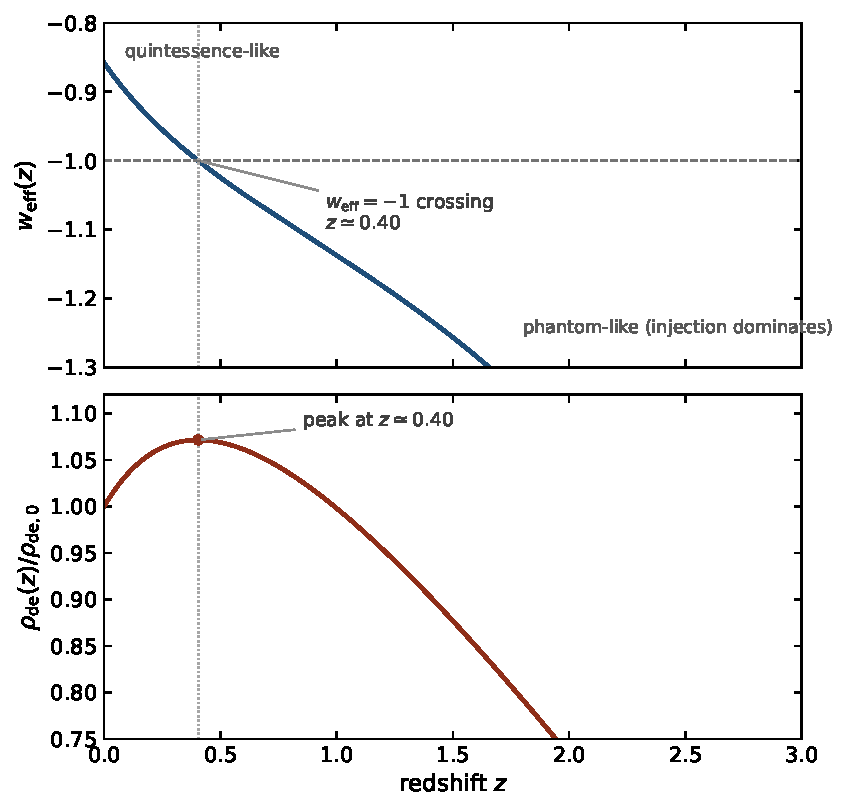
\includegraphics[width=0.62\textwidth]{figures/weff_history.pdf}
\caption{Best-fit history of the two-channel mechanism, obtained by integrating Eq.~(\ref{eq:master}) at the best-fit parameters of this section ($\mu_0=0.37$, $n=1.8$, $\kappa=0.85$). \emph{Top:} effective equation of state $\weff(z)$, crossing $w=-1$ from below at $z\simeq0.40$. \emph{Bottom:} dark-energy density in units of its present value, peaking at the crossing and declining thereafter; the crossing and the peak coincide by construction (Section~\ref{sec:ordering}).}
\label{fig:history}
\end{figure}

\textbf{Efficiency.} Although bounded by $\kappa\le1$ on energy grounds, $\kappa$ was fitted freely (allowed up to 40). The data select $\kappa\simeq0.85$. On the conservative vector the $\chi^2(\kappa)$ profile, with the other parameters re-optimised, is a shallow valley bounded above by the \lcdm{} value: $\mu_0\to0$ switches the mechanism off and recovers \lcdm{} ($\chi^2=17.6$) at any $\kappa$, so the profile cannot exceed it. Converged values are $\chi^2\simeq16.2$ at $\kappa=0.5$, $13.8$ at $\kappa=1$, and $\simeq17.2$ by $\kappa=3$, where the optimiser retreats to near-zero feeding. The free-$\kappa$ optimum sits at $\kappa\simeq1.01$ ($\chi^2=13.9$, Table~\ref{tab:fits}) --- effectively at the physical ceiling $\kappa=1$ --- and adding the supernova sample pulls the selected value to $\kappa\simeq0.85$, comfortably within it. Both lie within the profile's shallow minimum, and the mild shift reflects the supernovae's additional low-redshift leverage rather than any tension in the fit. The full improvement over \lcdm{} is available only in the neighbourhood of the physical budget.

\textbf{Statistical assessment.} $\Delta\chi^2\simeq6$ for three additional parameters is a $\sim2\sigma$-level preference on the data vector fitted here (first-release BAO with the Pantheon+ sample); the field-level preference has since strengthened to $2.8$--$4.2\sigma$ with DESI's second data release, depending on the supernova sample \citep{DESI_DR2}, and the completed five-year survey is under analysis \citep{DESI_completion}. Information criteria score the model roughly level with \lcdm{}. The mechanism reproduces the observed signal in shape and amplitude, leaves no significant residue for the empirical form to explain, and stands or falls with the signal as it matures.

\textbf{Perturbation-level check.} The best-fit $\weff(a)$ was tabulated and passed to the CAMB Boltzmann code \citep{CAMB} through its PPF module \citep{PPF}, which evolves perturbations stably across the $w=-1$ crossing, under the minimal completion of the interaction: homogeneous energy transfer and standard sound speed. The professional code reproduces this paper's background pipeline to $0.01\%$ in the BAO observables and to $0.01$ Mpc in the sound horizon. At fixed cosmological parameters the model's CMB TT spectrum differs from \lcdm{} by at most $+0.4\%$ at $\ell=2$--$10$ (late integrated Sachs--Wolfe, far beneath cosmic variance of tens of percent per multipole) and by $0.06\%$ through the acoustic peaks; the growth observable $f\sigma_8(z)$ differs by at most $2\%$ over $0<z<1.5$, against current measurement precision of $5$--$10\%$. The model therefore survives its first perturbation-level exposure, and neither the ISW tail nor structure growth discriminates it from \lcdm{} or $w_0$--$w_a$ at present precision: the discriminating data remain the expansion history itself.

% ----------------------------------------------------------------------
\section{Parameterisation artifacts}\label{sec:artifacts}

The $w_0$--$w_a$ form can manufacture crossings. Taking the $\kappa=0$ limit --- whose equation of state provably never drops below $-1$ --- at a data-allowed parameter point, generating mock observations, and fitting the mock with $w_0$--$w_a$ recovers $w_0=-0.97$, $w_a=-0.05$: an implied phantom crossing at $z\simeq1.2$ that the underlying model does not contain.

This bears on the proposal in two ways. It softens the empirical case for a genuine crossing, since part of any reported crossing can be an artifact of the two-parameter form; and it implies that a genuinely crossing model cannot be distinguished from a thawing non-crossing one by the $w_0$--$w_a$ numbers alone. The discriminating measurement is the full expansion history.

% ----------------------------------------------------------------------
\section{The matching problem}\label{sec:matching}

One physical choice carries the result: the injection shares its energy over the interior's physical volume ($\propto a^3$) rather than the parent's horizon volume. Under horizon-volume accounting the injection would scale with the boundary exactly as the dilution does, their ratio would freeze, and the crossing would vanish. Three results bear on the choice; one question remains open.

\textbf{The dilution channel is an identity.} The Misner--Sharp mass relation \citep{MisnerSharp1964} $M=\tfrac{4\pi}{3}\rho\,(a r_b)^3$ combined with the boundary-at-horizon condition $a r_b = 2GM/c^2$ gives $\rho = 3c^6/32\pi G^3 M^2$: density falling exactly as $M^{-2}$. The dilution term reproduces this slaving numerically to one part in $10^5$. It is the statement that the interior vacuum remains consistent with the horizon condition as the parent grows.

\textbf{The two channels are independent mechanisms driven by one mass function.} The injection and dilution terms are not two sides of a single conservation identity. Injection is energy transfer across the accreting boundary, set by the growth \emph{rate}: by Eq.~(2), $\mu_0 a^n\,M_p = dM_p/d\ln a$, so the injection term of Eq.~(3) is $\kappa\,(dM_p/d\ln a)/a^3$ (Appendix~\ref{app:vaidya}). Dilution follows independently from the horizon-slaving relation $\rho\propto M_p^{-2}$ (Appendix~\ref{app:ms}) and, unlike ordinary FRW dilution, is gated by feeding. Both channels are legitimately driven by the same $M_p$: in spherical symmetry the Vaidya mass function coincides with the Misner--Sharp mass.

\textbf{The exact matchings use interior-volume accounting.} The Oppenheimer--Snyder construction \citep{OppenheimerSnyder1939} --- the exact matching of an FRW interior to a black-hole exterior --- identifies the exterior mass with interior density times the interior's physical FRW volume, the quantity scaling as $a^3$. Energy that has crossed the horizon belongs to the interior's budget and dilutes with the interior's expansion; horizon-volume accounting would import the boundary's geometry into the interior's local bookkeeping, which the exact solutions do not do.

\textbf{The clock mapping is absorbed.} The relation between parent proper time and interior cosmic time is strongly nonlinear near a horizon and is not derived here. Because the feeding history is fitted as a free function of the interior scale factor, any monotonic re-mapping of clocks is absorbed into $(\mu_0,n)$: the ambiguity affects only the translation of the fitted history into the parent's own schedule, not any prediction on our side of the horizon.

\textbf{Open.} Oppenheimer--Snyder matches a dust interior across a comoving, non-feeding boundary. An actively fed horizon is Vaidya-like \citep{Vaidya1951} and the boundary advances as the parent grows; the strict junction analysis for that case \citep{Israel1966,BarrabesIsrael1991}, and the perturbation-level treatment, remain to be done. The question is sharp: does active feeding modify the interior-volume accounting the exact static matchings support?

% ----------------------------------------------------------------------
\section{Relation to prior work: what is new and what is not}\label{sec:prior}

The present mechanism differs from previous black-hole-cosmology proposals --- black-hole-interior models in general, holographic dark energy, and cosmologically coupled black holes --- in that the dark-energy evolution arises from the competition between an accretion-driven injection term and an accretion-driven dilution term sourced by the same feeding history.

\subsection{Existing ingredients}\label{sec:existing}

Black-hole-interior and bounce cosmologies constitute an established literature \citep{Pathria1972,NovelloBergliaffa2008,Poplawski2010}. A horizon-set vacuum density ($\rho\propto R^{-2}$) is the defining relation of the holographic dark-energy programme \citep{CohenKaplanNelson1999,Li2004}, which includes a published black-hole-universe realisation with a static horizon \citep{Gaztanaga2022}. Matter-to-dark-energy conversion by black holes has been published for holes within our universe \citep{CrokerWeiner2019}, including a 2024 result recovering the DESI time evolution from cosmologically coupled black holes \citep{Croker2024}. Claimed direct observational support exists --- supermassive black holes in elliptical galaxies growing $8$--$20\times$ beyond accretion, with zero coupling formally excluded at high confidence \citep{Farrah2023growth,Farrah2023coupling} --- and is contested by independent constraints from globular-cluster black holes \citep{Rodriguez2023}, Gaia binaries \citep{AndraeElBadry2023}, high-redshift AGN \citep{Lei2024}, and accretion histories \citep{Lacy2024}, with the underlying theoretical argument also disputed \citep{GaurVisser2024}. The question is unresolved. Finally, an effective phantom equation of state produced by energy injection into the dark sector is standard interacting-dark-energy physics \citep{DasCorasanitiKhoury2006,Wang2016}.

\subsection{Novel elements of the present mechanism}\label{sec:novel}

\begin{enumerate}
\item A single accretion flux sourcing \emph{both} an injection and a dilution channel, with their relative scaling fixed by geometry ($a^3$ against the boundary) rather than by choice.
\item The consequent theorem (Section~\ref{sec:ordering}) that the rise--peak--decline history and the past-only phantom phase are forced: the reverse ordering is unattainable for $\kappa\le1$.
\item The outward-facing (parent-hole) realisation of conversion-as-dark-energy, in which the one-way horizon that forbids $w<-1$ in the dilution-only limit is what licenses the injection.
\item The demonstration that this mechanism captures the full DESI+Pantheon+ evolving-dark-energy preference at the empirical parameterisation's fit quality, with the fitted efficiency landing inside the physical budget.
\end{enumerate}

% ----------------------------------------------------------------------
\section{Speculative extensions}\label{sec:speculative}

The following consequences arise from the broader black-hole-interior framework rather than from the fitted two-channel mechanism itself and may, if necessary, be discounted without prejudice to Sections~\ref{sec:model}--\ref{sec:prior}.

\textbf{A large-scale cutoff.} A universe bounded at the parent's scale cannot support fluctuations larger than the container. Implementing a hard primordial cutoff in the Boltzmann code quantifies the prediction and discriminates between geometric conventions. With the largest supported wavelength equal to $2\pi R_s$, the suppression is confined to the quadrupole and octopole ($D_2$ reduced to $79\%$ of \lcdm{}, $D_3$ to $95\%$, no effect beyond $\ell=4$) --- matching the location and shape, though only part of the amplitude, of the observed low-quadrupole anomaly \citep{Schwarz2016,PlanckIsotropy}. With the largest wavelength equal to the diameter $2R_s$, power is suppressed to $\sim35\%$ through $\ell\simeq5$ and $69\%$ at $\ell=7$: a broad shelf the data do not show, disfavouring that convention. Both variants recover \lcdm{} by $\ell=10$. One conditionality attaches: the container's comoving size, $R_s/a$, was vast early and is at its minimum today, so whether any cutoff imprints at all depends on whether modes must fit the instantaneous comoving cavity or only the container at their generation --- a boundary-condition question belonging to the junction analysis of Section~\ref{sec:matching}. Under the generation-epoch reading no cutoff arises.

\textbf{A preferred axis.} A rotating (Kerr) parent or uneven feeding would imprint a preferred direction, potentially connecting to reported large-angle CMB alignments \citep{LandMagueijo2005,Schwarz2016}. This is a qualitative expectation rather than a derived prediction: because the boundary is a temporal surface (\S\ref{sec:energyconditions}), anisotropy in the accretion flow enters the interior as a large-scale directional modulation rather than as local structure, which is the correct character for the observed low-multipole anomalies. Whether the amplitude matches requires the junction analysis of \S\ref{sec:matching} and is unexplored here.

\textbf{The efficiency deficit.} The fitted $\kappa\simeq0.85$ leaves $\sim15\%$ of the infalling rest energy unaccounted for by the vacuum channel. The constraint is loose ($\kappa=0.5$ costs only $\Delta\chi^2\simeq1.6$, $\sim1.3\sigma$), but the deficit has natural homes. Standard accretion physics radiates $6$--$42\%$ of rest energy in the parent's frame before matter crosses the horizon \citep{BardeenPressTeukolsky1972,NovikovThorne1973,ShakuraSunyaev1973}; a $15\%$ loss corresponds, under thin-disc assumptions, to a briskly spinning parent ($a_*\sim0.9$) \citep{Thorne1974} --- the same property that would imprint the preferred axis above, making the deficit and the axis potential fingerprints of a single parameter. Alternatively, for a rotating hole the swallowed energy genuinely partitions between irreducible (area) growth and rotational energy, so a share retained by the boundary is not excluded; and a small fraction may arrive as interior radiation rather than vacuum. The fitted model is agnostic among these homes: $1-\kappa$ is a catch-all for energy that does not become interior vacuum.

\textbf{Implications if correct.} Dark energy would be the vacuum energy of the region we inhabit, its magnitude set by the size of the object we live inside, its evolution the record of that object's accretion; the Big Bang a bounce; the cosmological ``constant'' not constant; the coincidence problem a statement about the parent's feeding history; the universe possessed of a boundary, a parent, and plausibly a lineage. The scale of these implications bears on the model's interest, not on its probability; the probability rests on Sections~\ref{sec:data} and \ref{sec:matching}.

% ----------------------------------------------------------------------
\section{Conclusion and decisive tests}\label{sec:conclusion}

Two channels forced by one one-way feeding --- energy delivered inward, a boundary pushed outward --- generate a dark energy that rises, peaks, and declines, crossing $w=-1$ without phantom matter, in an order the model cannot reverse. Fit to Planck, DESI, and the full Pantheon+ sample, the mechanism matches the empirical description of the evolving-dark-energy signal to within rounding, places the crossing and the peak where the data put them, and selects a conversion efficiency inside the physical budget. The dilution channel is the Misner--Sharp identity; the injection accounting follows the exact Oppenheimer--Snyder matching; the clock ambiguity is absorbed by the fitted history.

Two tests decide it. Theoretically: the junction analysis for an actively fed (Vaidya-type) boundary, on which four separate questions now converge --- the interior-volume accounting that generates the crossing, the partition of swallowed energy between interior and boundary, whether the large-scale cutoff of Section~\ref{sec:speculative} imprints at all, and the profile and normalisation of the flux whose field-theoretic realisation (Section~\ref{sec:energyconditions}) remains open. Empirically: the first-pass Boltzmann implementation reported in Section~\ref{sec:data} (tabulated $\weff(a)$ through PPF, perturbations stable across the crossing, pipeline validated against CAMB to $0.01\%$) should be extended to a full likelihood analysis over the complete Planck, DESI, and supernova datasets with the interaction's perturbation sector derived rather than assumed minimal --- and beyond that, the evolving-dark-energy signal itself, strengthened across DESI's releases from $\sim2\sigma$ to $2.8$--$4.2\sigma$ \citep{DESI_DR2}, will either mature into a measurement or dissolve. The model makes one bet --- that the signal is real and has the two-channel shape --- and it is stated precisely enough to lose.

% ----------------------------------------------------------------------
\section*{Acknowledgements}

The hypothesis, conceptual development, research direction, and all analytical and interpretive decisions are the author's own. The author directed the work throughout --- identifying the problems, driving the successive refinements of the model, and adjudicating every result. Claude (Anthropic) served as an instrument of that direction, formalising the mathematics, performing the computations, and drafting the text, and equally as an adversary, pressuring the author's proposals on physical and statistical grounds so that ideas were retained only after surviving challenge; several key turns in the model's development followed from the author overriding or correcting the tool. The general-relativistic scoping of Appendices A--C, and an independent reproduction of the numerical pipeline as a validation check, were developed through the same directed, adversarial dialogue with ChatGPT (OpenAI). All scientific interpretations and conclusions remain the author's sole responsibility.

{\sloppy\vspace{0.5em}\noindent\textbf{Data and code availability.} The analysis pipeline, reproduction scripts, and this manuscript's source are available at \url{https://github.com/ChrisPGreen/two-channel-dark-energy}, archived at Zenodo, \texttt{doi:10.5281/zenodo.XXXXXXX}.\par} The supernova data are the public Pantheon+ release; DESI and Planck inputs are as cited.

% ----------------------------------------------------------------------
\appendix

\section*{Appendices}
\addcontentsline{toc}{section}{Appendices}
\noindent\textit{Supporting derivations for the two-channel mechanism.}

\section{The injection channel from the Vaidya flux}\label{app:vaidya}

The ingoing Vaidya metric, $ds^2=-\left(1-2GM(v)/c^2 r\right)dv^2+2\,dv\,dr+r^2 d\Omega^2$, carries the stress tensor $T_{ab}=\big[\dot M(v)/4\pi r^2\big]\,k_a k_b$ with $k_a$ null \citep{Vaidya1951}. The total energy crossing any sphere during $dv$ is $\oint T_{ab}k^a k^b\,dA\,dv = dM$ \emph{exactly}: the $r^{-2}$ of the flux cancels the sphere area, so the transfer is a global increment with no preferred angle and no locally defined ``amount per place.'' The physically available source strength is therefore set by the growth \emph{rate} $\dot M_p$, not by the accumulated mass. Eq.~(3) already respects this: by Eq.~(2), $\mu_0 a^n\,M_p(a)=dM_p/d\ln a$, so the injection term is $\kappa\,(dM_p/d\ln a)/a^3$ --- the rate law in volume-distributed form. Distributing $dM_p$ over the interior physical volume $V\propto a^3$ then yields the $a^{-3}$ scaling; no alternative exponent arises without relocating where the injected energy resides (Appendix~\ref{app:conversion}).

\section{The dilution channel from horizon slaving}\label{app:ms}

The Misner--Sharp mass \citep{MisnerSharp1964} of a spherically symmetric spacetime is $M_{\rm MS}=(c^2 R/2G)\big(1-g^{ab}\nabla_a R\,\nabla_b R\big)$, and an apparent horizon sits at $R_A=2GM_{\rm MS}/c^2$. For an interior whose vacuum density is set by the horizon condition, $M=\tfrac{4\pi}{3}\rho R_A^3$ fixes $\rho=3c^6/32\pi G^3 M^2$, whence $d\ln\rho/d\ln M=-2$ identically: $\dot\rho_{\rm dil}=-2\,(\dot M_p/M_p)\,\rho$. Two properties matter. The coefficient is geometric, not fitted; and the channel is \emph{gated by feeding} --- if accretion stops, $\dot M_p=0$ and dilution ceases --- distinguishing it from ordinary FRW volume dilution ($-3H\rho$), which plays no role for this horizon-slaved component. In spherical symmetry the Vaidya mass function coincides with the Misner--Sharp mass, so a single $M_p$ legitimately drives both this channel and that of Appendix~\ref{app:vaidya}.

\section{Scope of the junction analysis and the rapid-conversion limit}\label{app:conversion}

Three layers separate the parent's accretion from Eq.~(3). (i) Parent-spacetime accretion (Appendix~\ref{app:vaidya}) fixes what crosses the boundary: $dE=dM_p$. (ii) Junction matching \citep{Israel1966,BarrabesIsrael1991} fixes the surface stress-energy induced on the null boundary --- an intrinsically two-dimensional quantity. (iii) Conversion and redistribution turn that boundary energy into a smooth interior source; this is transport physics beyond junction theory, and it is the open conversion vertex of \S\ref{sec:energyconditions}. Symmetry cannot settle layer (iii): spherical symmetry does not imply homogeneity --- a thin shell $\rho\propto\delta\big(r-r_s(t)\big)$ is perfectly isotropic yet maximally inhomogeneous --- so matching conditions alone determine what reaches the boundary, not how the interior fills. The minimal completion is a reservoir, $\dot\rho_X = Q-\Gamma\rho_X$, $\dot\rho_{\rm de}=\Gamma\rho_X - D$, with $\Gamma^{-1}$ the conversion time; the present paper is the rapid-conversion limit $\Gamma\gg H$. A finite $\Gamma$ introduces a memory kernel whose smearing is largely absorbed into the fitted history $(\mu_0,n)$ at background level, but a delay comparable to $H^{-1}$ would desynchronise the channels --- dilution responds to horizon growth immediately, injection to past accretion --- and could modify the strict form of the ordering theorem (\S\ref{sec:ordering}); that the data are captured by a two-parameter history with no memory freedom is circumstantial evidence against a large delay. The motivation for $\Gamma\gg H$ is the model's own ontology (\S\ref{sec:energyconditions}): the dark component is horizon-coupled rather than transported, and flux across a boundary whose causal role is temporal enters distributed in space and localised in time.

\bibliographystyle{unsrtnat}
\bibliography{references}

\end{document}
